%!TEX = xelatex
\documentclass[conference]{IEEEtran}
\IEEEoverridecommandlockouts
\usepackage[style=ieee]{biblatex}
    \addbibresource{references.bib
}
\usepackage{graphicx}
\usepackage{amsmath}
\usepackage{amssymb}
\usepackage{xcolor}
    \newcommand{\todo}[1]{\textcolor{red}{[ #1 ]}}
    \newcommand{\instruction}[1]{\textcolor{orange}{#1}}
% \renewcommand{\todo}[1]{} % Uncomment to hide todos.
% \renewcommand{\instruction}[1]{} % Uncomment to hide instructions.

\newcommand{\hidden}[1]{}

\usepackage[colorlinks=false]{hyperref}

\title{STATS 402 - Interdisciplinary Data Analysis\\
    Resource-Constrained Deep Reinforcement Learning for Battlesnake
}
\author{\IEEEauthorblockN{Steven Hé (Sīchàng)\\
    sichang.he@dukekunshan.edu.cn
}}

\begin{document}
\maketitle

\begin{abstract}
    \instruction{Insert a very brief paragraph describing your project (300 words)}

    \todo{the actual problem you are considering and the motivation behind your method;}

    \todo{brief description of the method you designed;}

    \todo{brief description of how you validated the method you proposed.}
\end{abstract}

\section{Introduction}

\todo{briefly introduce the background knowledge of the actual problem
    you want to solve and the motivation behind your design
}

\todo{briefly introduce the characteristics of your method}

Battlesnake~\cite{battlesnake}
is a popular online programming competition in the form of a simultaneous
multiplayer board game. Similar to the arcade snake game,
each player controls a snake in real time on a finite grid board to be the last
one alive; the snake can change directions within each turn,
grow in length by eating randomly spawned food,
die from colliding with walls or snake bodies,
or starve to death after not eating for a long time (100 turns),
as demonstrated in Fig.~\ref{fig:game}.
Instead of having human players control the snakes, in Battlesnake,
players develop a computer program to control their snakes' directions in each
turn, by implementing a web server that responds to the game server's request,
which contains the entire game state.
This means players can implement their algorithms freely,
as long as they can finish the response within the time limitation (500ms).

\begin{figure}
    \centering
    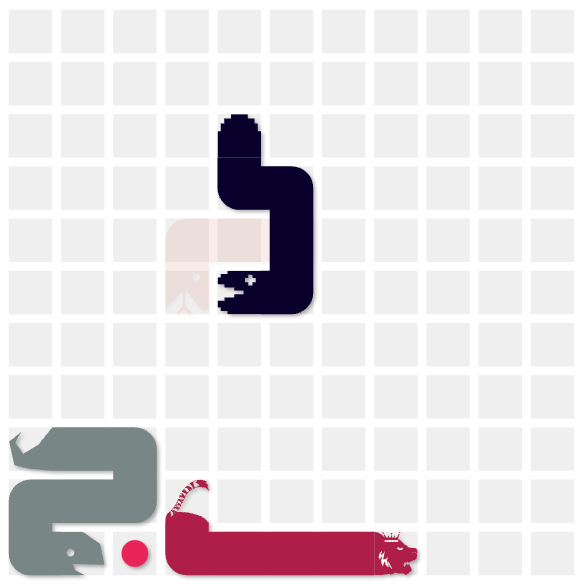
\includegraphics[width=\linewidth]{snake_game_screenshot.png}
    \caption{A Standard Battlesnake Game with 4 Snakes on A 11x11 Board.
        The transparent snake is already dead.
    }
    \label{fig:game}
\end{figure}

Battlesnake is an ideal target for implementing deep reinforcement learning.
Traditionally,
the leader board is occupied by players employing various heuristics and Monte
Carlo tree search algorithms,
most notably minimax~\cite{hill2018building,binnersley2020battlesnake}. However,
more recently,
even well-defined heuristics and tree search algorithms are only adequate for
intermediate-level gameplay~\cite{schier2019adversarial}. Additionally,
given the large search space (over $(3^n)^t$ raw possibilities for $t$ turns in
a game with $n$ snakes),
tree search algorithms are computationally demanding even when techniques like
alpha-beta pruning are employed. This cost problem is magnified,
especially considering the game sets a 500ms action time limit.
To address these problems, we compare Battlesnake to the game of Go,
which also has a large possibility space and potentially long time horizon,
and AlphaGo has demonstrated that deep reinforcement learning can excel in such
situations and achieve superhuman-level performance~\cite{silver2016mastering}.
More recent examples of deep reinforcement learning systems acing video games
include OpenAI Five defeating human world champions in Dota 2,
a much more complicated online multiplayer battle game~\cite{berner2019dota}.
Therefore,
it is sensible that deep reinforcement learning can possibly be employed to
build state-of-the-art Battlesnake agents.

A deeper aspect to explore is developing deep reinforcement learning agents to
operate in resource-constrained environments.
Most Battlesnake players are amateurs hosting their web servers on cheap VMs on
cloud platforms or Raspberry Pi computers~\cite{standard_leaderboard}.
Similar to these resource-constrained environments, use cases,
such as autonomous spacecraft control,
have seen deep reinforcement learning applied in
them~\cite{harris2022generation}. More closely related,
proximal policy optimization (PPO)~\cite{schulman2017proximal},
the same deep reinforcement learning technique employed by OpenAI Five,
has been successfully deployed in compute and memory-limited robotic control,
specifically quadrotor navigation~\cite{huang2023collision,hegde2023hyperppo}.
Thus,
developing a deep reinforcement learning Battlesnake agent capable of operating
on low-capability devices, like low-tier cloud VMs and Raspberry Pis,
should be feasible;
such solutions would also demonstrate more fairness and practical contributions
among the competition.

\todo{present the organization of the subsequent part of the article}

\subsection{Related Work}

\todo{analyze and summarize the existing methods in the field related to the
    problem you are considering
}

\todo{explain the advantages and disadvantages of the existing methods}

As shown by AlphaZero~\cite{silver2017mastering},
a deep reinforcement learning agent can learn,
with no other knowledge about the game than only a simulation environment,
is already enough to achieve superhuman performance in many board games.
However,
AlphaZero was built with a massive neural network and trained using 4000 TPUs,
a condition unthinkable for the ordinary Battlesnake players. Meanwhile,
prior Battlesnake implementations utilizing reinforcement learning often also
incorporate heuristics and tree search,
instead of relying purely on reinforcement learning
algorithms~\cite{chung2020battlesnake,binnersley2020battlesnake}.

\todo{explain the differences and characteristics of your approach relative to
    the existing methods
}

we are interested to learn how well such purely
deep-reinforcement-learning-based agents can perform.

\section{The Proposed Method}

\instruction{In this part, you need to describe your method in detail.
    According to the specific problems considered in the article and the
    characteristics of the method designed,
    the content that may be included is problem statement and assumptions,
    initial data analysis,
    an introduction to the general procedure of your method and the
    corresponding flow chart, etc.
}

We propose to develop a purely deep-reinforcement-learning-based Battlesnake
agent capable of operating in resource-constrained environments.

The agent will be developed by referencing open-source implementations
in~\cite{siddiqui2020multiagent,chung2020battlesnake,wrenger2024rusty}.
It will be designed to compete in the standard Battlesnake game on an 11x11
board with 4 competing players.

\paragraph{Feature Extraction}
Feature extraction will follow the basic methods
in~\cite{siddiqui2020multiagent,archinukmonte}, with some adjustments.
Specifically,
we will pad the board to a 21x21 grid and rotate it so that the snake's head is
centered and faces up. Therefore,
the three valid actions for the snake would be ``up'', ``left'',
and ``right'' only.
We ignore opponents' health because snakes hardly starve in
practice~\cite{siddiqui2020multiagent}.
We will have 10 layers of 21x21 matrices ($\mathbb R^{10\times21\times21}$),
with each entry normalized to be within $(-1,1)$, and 0 indicating emptiness:
\begin{itemize}
    \item Wall layer. 1 indicates that the position is out of bound.
    \item Our snake's body layer.
        The value of each of our body segment position will be calculate as $$
            v_b:=\frac{2L_{\text{rest of body}}-1}{239}
        $$ where $L$ is the length of the snake.
        Large $v_b$'s indicate the position would remain occupied for longer.
        The tail always corresponds to a $v_b<0$ for distinction.
    \item Three opponent snakes' layers.
          These layers will be sorted by the opponents' length and then health.
          Each opponent snake will be represented by 2 layers. \begin{itemize}
              \item Head layer. The value of each head will be calculated as $$
                        v_h:=\frac{1+2(L_{\text{opponent}}-L_{\text{us}})}{239}.
                    $$ $v_h>0$ indicates that the opponent snake is at least as
                    long as our snake,
                    so colliding with their head would kill our snake;
                    $v_h<0$ indicates the opposite.
              \item Body layer. This layer will also be calculated using $v_b$.
          \end{itemize}
    \item Food layer.
          The value will be $\displaystyle\frac{101-H_{\text{us}}}{100}$ if
          there is food in the position.
          A large value indicates our snake is hungry.
\end{itemize}

We design the reinforcement learning reward based on the outcome of the game.
The reward will be 1 if our Battlesnake agent wins, or -1 if it loses.
To speed up training convergence,
we will also apply a reward of 0.002 for each turn survived,
following the practice in~\cite{chung2020battlesnake}.

\paragraph{Neural Network Model}
The reinforcement learning training will be done using
PPO~\cite{schulman2017proximal}.
We choose PPO because of its flexibility and high empirical performance in
adversarial games,
as observed
in~\cite{berner2019dota,binnersley2020battlesnake,chung2020battlesnake}.
During training, we will simulate self-play games with four players,
each controlled by our agent.
To optimize our agent for competing against different levels of opponents,
each player of the simulated game will have a 20\% chance of being controlled by
an older version of our agent,
similar to the setting in~\cite{silver2017mastering}. However,
to avoid useless simulations,
we will reassign the players if all of them are older versions.

\section{Performance Evaluation}

\todo{introduce your method of verifying the validity/correctness of your method}

\subsection{Evaluation Environment and Research Questions}

Specify, we raise the following questions.

\paragraph{How well can a purely deep-reinforcement-learning-based agent
    perform?
}

\paragraph{How to strive a balance between fast inference time and high model
    capability?
}
We aim to develop our agent to be capable of operating on resource-constrained
environments,
akin to the low-tier VMs and Raspberry Pis other Battlesnake players deploy
their agents on. For our purpose,
we will target a standard VM provided by Duke University,
which has two Intel Xeon 6248R CPU cores and 3.6GiB of RAM;
this CPU is roughly twice as powerful as a Raspberry Pi 5's CPU\footnote{See
    \url{https://www.cpubenchmark.net/compare/3732vs5893/Intel-Xeon-Gold-6248R-vs-ARM-Cortex-A76-4-Core-2600-MHz}.
}. However, we also target a high performance in the game. Therefore,
we need to design the neural network of the agent,
such that the agent utilizes as much time as possible when performing inference.

\subsection{Implementation}

\subsubsection{Feature Extraction Implementation}

The Pettingzoo environment has been implemented based on the feature extraction
described in the
proposal\footnote{\url{https://github.com/SichangHe/STATS402_course_project/tree/main/battlesnake_train/battlesnake_gym}}.
This environment has been wrapped using SuperSuit and tested against Stable
Baselines3 APIs,
and appears to be working properly as a Stable Baselines3 environment in our API
unit testing.

Game simulation is powered by the implementation in~\cite{wrenger2024rusty},
which leads to two challenges. First, the game simulation is written in Rust,
while the Pettingzoo environment needs to be in Python. To bridge this gap,
we leverage a mature Rust-Python interoperability solution,
the PyO3 library~\cite{pyo3} and the build tool Maturin~\cite{maturin}.
A wrapper Rust struct is created and registered as a Python class to represent a
Battlesnake game,
and provide methods for the Pettingzoo environment to interact with.
Another Python class (\textsf{BattlesnakeEnv})
then wraps the Rust struct and implements the Pettingzoo Parallel API. Second,
the game simulation only presents the original board state,
without any transformations based on each snake agent's position or orientation
like we had planned. Therefore,
we referred to the feature extraction implementation
in~\cite{siddiqui2020multiagent},
and reimplemented our similar approach in Rust.

To be more specific,
the feature matrix of $\mathbb R^{9\times21\times21}$ is constructed in Rust and
converted into a Numpy array~\cite{harris2020array}
to suit the methods in \textsf{BattlesnakeEnv}. Notably,
the features are nine layers instead of ten,
as incorrectly stated in the proposal; layer 0 represents walls,
layers 1 represents the agent's body, layer 2, 4,
6 represent the head of each opponent snake, layer 3, 5,
7 represent the body of each opponent snake, and layer 8 represents food.
To implement our proposed feature extraction,
we first construct three intermediate values:
each snake's body layer on the original board,
the order of the snakes based on their length and health,
and the head values of ordered opponent snakes from each snake's perspective.
We then calculate the full feature matrix for each snake's observation without
the rotation, and the facing of each snake. Finally,
these two values are sent to Python,
where we conveniently construct the final feature matrix by rotating the feature
matrix in Numpy according to the snake's facing. In this process,
a large number of indexing is used to construct the feature matrix,
causing difficulties to debug. Though,
we tested the implementation by inspecting the intermediate values,
confirming its correctness.

Besides feature extraction,
the Rust implementation also converts relative actions input from the Python
side into absolute actions for the game simulation. For example,
if an agent's head is facing ``left'' and the relative action they output is
``right'',
our implementation converts the action to ``up'' before sending it to the game
simulation.
This facing detection is based on the relative position of the agent's head and
second body part. The four orientations ``up'', ``right'', ``down'',
and ``left'' are represented as integers 0, 1, 2, 3, respectively,
in a clockwise order.
Both the action input $A_{relative}$ and the facing detection $F$ use this
representation, so the absolute action $A_{absolute}=(A_{relative}+F)\bmod 4$,
and the facing can be directly used for the rotation in Numpy mentioned above.

\subsubsection{Neural Network Implementation}

We plan to develop our neural network gradually to fit the computation budget.
We will first use a simple multilayer perceptron (MLP)
to validate our PPO approach. Then,
we will design a more complicated neural network that can reliably perform
inference within 440ms on a standard Duke VM.
We choose to aim at 440ms because the average ping from the VM to the
Battlesnake website is around 20ms,
and we reserve three times that amount for network out of the 500ms allocated
action time. We will train the agent on a server with a GPU.

We will base our training implementation on the successor of OpenAI
Gym~\cite{brockman2016openai} called Gymnasium~\cite{farama2024gymnasium},
and Stable Baselines3~\cite{raffin2024stable}.
We will implement an Gymnasium gym environment based on the implementation
in~\cite{chung2020battlesnake},
and utilize the PPO implementation in Stable Baselines3 to train our agent.
Since these packages do most of the heavy-lifting,
this implementation should be feasible even though the training algorithms are
non-trivial.

Following our plan,
we constructed more complex and larger neural networks to better extract
features from the game board. The main models include a VGG-like model,
a deeper MLP model, and small and big Vision Transformer (ViT) models.

\paragraph{VGG-like Model}
We constructed convolutional neural network (CNN) layers for feature extraction,
referencing the VGG16 model~\cite{simonyan2014very}.
Our feature layers consist of the first 7 convolutional layers,
the first 3 max-pooling layers, and the adaptive average layer in VGG16,
incrementally compressing the input feature matrices from $\mathbb R^{9\times
            21\times 21}$ to $\mathbb R^{256\times 2\times 2}$.
The features are then flattened and fed into 3-layer MLPs with hidden layer
widths 256 for either policy or value networks.
Our implementation references the PyTorch~\cite{paszke2019pytorch}
VGG16 model implementation.

We constructed a shallower and thinner model than the VGG16 model primarily for
two reasons: our feature matrices are smaller,
and our compute resources are limited.
We only used the first 3 max-pooling layers because our feature matrices have
width 21 instead of the 224 in VGG16. That is,
after all 5 max-pooling layers with kernel size 2 in VGG16,
the feature matrices would be compressed from width 224 to 7; in comparison,
our feature matrices are compressed from width 21 to 2 after 3 similar
max-pooling layers.
Additionally, we believe that the game board of Battlesnake is simple enough,
that $256\times 2\times 2=1024$ numbers are sufficient to extract the features,
and MLP layers with width 256 are sufficient to learn these smaller features.

After initial testing, the VGG-like model performed poorly,
therefore we added a residual layer to it.
Our reasoning is the CNN layers may lose the positional information,
e.g., the snake's head is always at the center of the feature matrices;
also, the network's larger depth might result in the vanishing gradient problem.
The residual is a 2-layer MLP with hidden layer of width 2048,
transforming the input features from $\mathbb R^{9\times 21\times 21}$ to
$\mathbb R^{1024}$ before adding them to the output of the CNN layers.

\paragraph{Deeper MLP Model}
Besides the VGG-like model,
we also constructed a deeper MLP model to test the performance of simple
feed-forward neural networks.
Our deeper MLP consists of a feature extractor with 4 hidden layers of width
1024 and a residual layer,
as well as separate 3-layer MLPs for either policy and value network,
with hidden layer width 512 and 256.

\paragraph{Vision Transformer (ViT) Models}
Since the ViT model has shown great success in image classification tasks as an
alternative to CNN models,
we constructed small and big ViT models for feature extraction.
Our small ViT model has patch size 7, 4 encoder layers, 4 heads, hidden size 256,
and MLP size 512.
It is modified to override the convolutional kernel to have input channel size 9
instead of 3,
because our feature matrices have 9 channels instead of the 3 used in image
classification.
Our big ViT model has patch size 3, 8 encoder layers, 8 heads, hidden size 512,
and MLP size 1024.

\subsection{Training Customization}

We directly customized the training loop in Stable
Baselines3~\cite{raffin2024stable}
to simplify the logic and prepare for the implementation to train the agent
against older versions of itself for 20\% of the time.
Because Battlesnake is a multi-player simultaneous-move game,
and Stable Baselines3 only supports single-agent environments,
previously, we created our environment
following the Pettingzoo~\cite{terry2021pettingzoo} parallel environment API,
and used SuperSuit~\cite{SuperSuit} to wrap it.

However, using SuperSuit for wrapping introduces two major downsides. First,
complexity is massively increased,
as SuperSuit requires multiple layers of wrappers.
This obstructs the understanding of the training process and hinders any
modifications to it, such as the old-version self-training. Second,
SuperSuit produces empty observations and zero rewards for dead agents,
so they appear alive,
and the environment appears to be a Stable Baselines3 vectorized environment.
These useless padding not only wastes computation during training,
but raises uncertainty.
Since dead agents' actions are counted into the number of steps the model has
trained, it is unclear how many steps the model has actually trained.
Additionally, it is unclear how the padding affects the training.

We modified and overrode the training methods on Stable Baselines3's PPO
implementation. Our implementation tracks each agent's statistics separately,
and only pushes them to calculate the returns and advantages when the agent
dies. We also correctly count the number of steps the model has trained,
by summing the number of steps each alive agent moves.
Although our implementation is not vectorized,
it still uses all available CPU cores on our server with dual EPYC 7763 64-Core
processors. Training for $16^5$ steps took 3777 seconds,
longer than the 3060 seconds the previous implementation took. However,
we note that the previous training was counting padding steps,
meaning that the new implementation has effectively trained more steps.

\subsection{Training Setup Modifications}

We realized the default entropy coefficient of 0 in the Stable Baselines3
implementation has been used,
causing insufficient exploration and convergence to spinning. Therefore,
we tried different entropy coefficients for the small and big ViT model.

In our inspections,
we found that the model does not seem to be interested in eating food,
and sometimes even starves to death with food nearby,
so we added a tiny reward bonus $R_e$ for eating food:
$$
    R_e = f_e(101 - h)
$$
where $f_e:=10^{-6}$ is a scaling factor and $h\in\{1,\ldots,100\}$ is the
snake's health before eating.
The rationale is to encourage the snake to eat food when its health is low,
since having a higher health give the snake more chances to survive.

Another modification is a fix to the loading of previous models.
We found that an index error in the loading process caused loaded previous
models to be cached with the wrong indices. This error caused two major issues:
large amounts of training time is wasted loading previous models due to cache
misses;
the model is sometimes not trained against the correct older versions of itself.
After fixing this issue,
we had another issue of running out of VRAM due to the large number of models
cached; we solved this issue by reducing the cache size to $32$.

We suspected that the incorrect implementation previous model loading resulted
in the strategy collapse of our models,
so we retrained the small ViT model after fixing the issue. However,
the model still converged to spinning after $100\times 16^4$ steps of training.
Therefore,
we decided that training against older versions of the model is indeed
insufficient to prevent strategy collapse,
and we have to rely more on adding larger entropy bonuses to encourage
exploration.

We decided to continue training the previous models after fixing loading the
previous models and added the food reward.
We continued training the big ViT model trained for $108\times 16^4$ steps,
and the small ViT model trained $192\times 16^4$ steps.
After training the small ViT model for $198\times 16^4$ steps and the big ViT
model for $208\times 16^4$ steps,
we also change their entropy coefficient from 0.01 to 0.1,
because the small model is spinning and the big model often circles around the
board.

\subsection{Technical Route Adjustments}

Although we planned to use the Gymnasium environment
library~\cite{farama2024gymnasium} in the proposal~\cite{proposal},
we found that it does not support multi-agent environments like the ones we have
in Battlesnake. Therefore,
we adjusted the environment library choice to
Pettingzoo~\cite{terry2021pettingzoo} instead.
Pettingzoo supports simultaneous-move multi-agent environments via its Parallel
API\footnote{\url{https://pettingzoo.farama.org/api/parallel/}},
and can be made compatible with Stable Baselines3~\cite{raffin2024stable}
using SuperSuit~\cite{SuperSuit}.

To benchmark our agent,
we propose to use the snake named ``ich heisse marvin'' as our comparison
target. \emph{ich heisse marvin}~\cite{wrenger2024rusty}
is an open-source tree search Battlesnake implementation.
It recently consistently ranks top 8 in the standard leaderboard,
despite being deployed on a Raspberry Pi. Its strategy utilizes
max\textsuperscript{n} and alpha-beta pruning.
We plan to let different versions of our agent play against \emph{ich heisse
    marvin} and calculate the win rate,
so that we can evaluate its performance over time.

As an additional evaluation,
we will deploy our agent on a standard Duke VM and join the standard
leaderboard~\cite{standard_leaderboard} to play against other players' snakes.

\todo{demonstrate the corresponding experimental results}

\subsection{Results}

We implemented the \textsf{render}
method on the environment to visualize the game.
The implementation produces ANSI colored text-based information on both the game
board and each agent's health.
By repeatedly calling the model to predict the next actions,
a terminal-based animation is created for ease of manual inspection.

\subsubsection{Manual Inspection}

\paragraph{Basic Model}

We tested the environment with the built-in multilayer perceptron (MLP)
policy from Stable Baselines3~\cite{raffin2024stable}.
For both the actor and the critic,
the MLP has two hidden layers of size 64 with ReLU activation.
Training the model on an M1 MacBook for 1,000,000 steps took 8 minutes 37
seconds, while leveraging most of the CPU cores.

After removing entirely the rewards and other parameters for the dead agents,
the results are much more reasonable. Based on manual inspection,
the agents are now able to avoid walls,
interestingly by circling the grid in a counter-clockwise manner,
as demonstrated in Fig.~\ref{fig:render2}. However,
they still do not seem to be able to avoid colliding with each other.
The agents also seem to be agnostic about food,
which is likely due to the lack of direct rewards for eating food. Overall,
the fact that the agents are able to avoid walls is promising,
indicating that they should be able to learn more complex strategies with a more
sophisticated model.

\begin{figure}
    \centering
    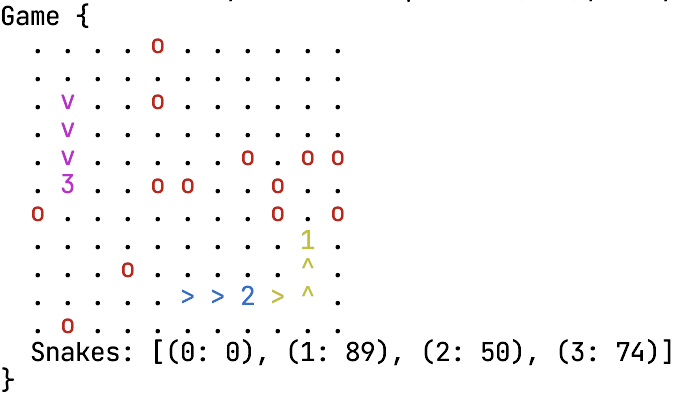
\includegraphics[width=\linewidth]{game_render_eg2.png}\\[12pt]
    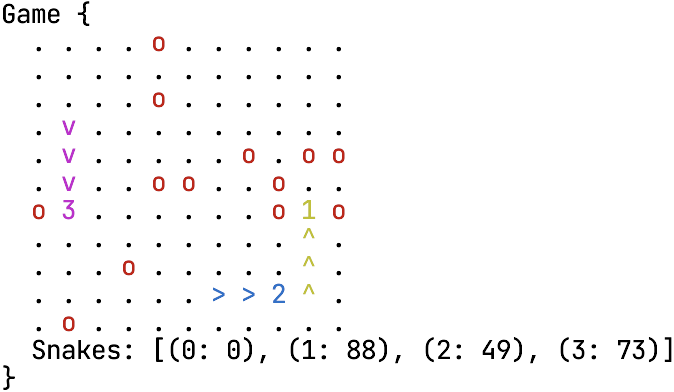
\includegraphics[width=\linewidth]{game_render_eg3.png}
    \caption{ANSI rendering of the game simulation after removing return values
        for dead agents. The lower figure is one step after the upper figure.
    }
    \label{fig:render2}
\end{figure}

We also inspected the behavior of a model trained for 100,000 steps.
This model does not yet seem to be able to avoid colliding with walls.
After training for 1,000,000 steps,
the model is able to avoid walls by circling the grid in a clockwise manner,
opposite to the previous case. Therefore,
it seems that the model needs more training steps to learn proper behaviors,
and an easily reachable local optimum is circling the grid.

\paragraph{VGG-like Model}
The VGG-like model took around 2000 seconds to train for $16^4$ steps using all
CPU cores on the aforementioned server,
about 10 times longer than the MLP model. However, it performed poorly,
even after we added the residual layer, and trained for $51 \times 16^4$ steps.
During manual inspection, the model cannot even consistently avoid walls,
which we consider a rudimentary learning task.
We suspect that the convolutional layers loose the positional information,
which is particularly significant in our case,
because our feature extraction steps center the snake's head in the feature
matrices. Alternatively,
another great possibility is the model requires much more training steps due to
its significantly larger size. Though,
we gave up on further training the VGG-like model because of the known
limitations of CNNs that they require a large amount of data to train.

Although we worried about the size of the model impacting the inference speed,
inference only took less than 1.0 millisecond and 600\,MiB of RAM on the default
Duke VM. Therefore,
we believe inference speed is not a bottleneck even on compute-constrained
environments,
but the size of the model will become a bottleneck when RAM is limited.
As a conclusion,
larger and more resource-intensive models like transformer are likely feasible,
with the training process being the major bottleneck.

\paragraph{Model without Entropy Bonus}
If trained without any entropy bonus,
larger models have a tendency to instruct the snake to spin in a circle
(Figure~\ref{fig:render}).
The deeper MLP model converged to go in a tight circle by keep turning left,
after less than $3\times 16^4$ steps, and all future models remained so.
Similarly,
we observed that the ViT model stays in a tight left-turn circle when the
snake gets into certain positions,
after the model is trained for $72\times 16^4$ steps.
Convergence to spinning happens because of lack of exploration.
At the beginning of training,
the model cannot avoid walls or other snakes consistently,
therefore spinning produces better results than moving around because it avoids
running into walls or snakes, despite making the snake starve to death.
Since there is no entropy bonus,
the model never has a chance to explore better moves,
and eventually converges to spinning.

\begin{figure}
    \centering
    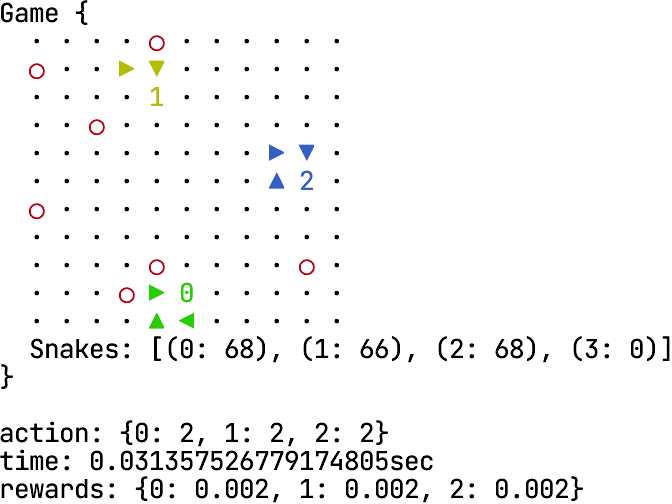
\includegraphics[width=\linewidth]{vit_spin_render.png}
    \caption{Game rendering with the small ViT model spinning in a circle.
    }
    \label{fig:render}
\end{figure}

\paragraph{Model with Entropy Bonus}
We tried to encourage exploration by adding an entropy bonus to the model.
However, after setting the entropy coefficient to 0.1,
our small ViT model could not learn to avoid walls even after training for
$32\times 16^4$ steps. Therefore,
we decided to lower the entropy coefficient to 0.01,
which resulted in our ViT model learning to spin again,
but reach for food when its health is low.
The deeper MLP model learned to spin after sufficient training,
no matter the entropy coefficient.

After we fixed the loading of previous models, added the food reward,
and increased the entropy coefficient to 0.1,
we trained the small ViT model for $587\times 16^4$ steps and the big ViT model
for $339\times 16^4$ steps (counting previous steps trained). However,
the small ViT model still has a less intense tendency to spin,
while neither models can avoid walls or themselves consistently.
Training the small ViT model for $16^4$ steps on an RTX 3090 takes around 580s,
and training the big ViT model for $16^4$ steps takes around 1300s.
We note that the major bottleneck in training is the training efficiency and
getting enough training steps for the model to converge.

\subsubsection{Comparison with Monte Carlo Tree Search}

For the results,
we anticipate the agent to have decent performance compared to tree-search-based
agents. Our agent's win rate against \emph{ich heisse marvin}
should grow as the training process goes on,
and eventually stabilize at a level slightly higher than \emph{ich heisse
marvin}'s. The agent should also be competitive in the standard leaderboard,
and reach top 20 given enough time.

We attempted to test the models against the tree search agent. However,
the tree search agent does not make simple mistakes like running into walls or
itself when it has a choice,
therefore the models can never win against the tree search agent in our
observation. We suspect this is why~\cite{chung2020battlesnake}
does not use standard agents as comparison and rather compare the models against
themselves. For the above reason,
we will not evaluate the models against the tree search agent,
but rather against other models.

\todo{analyze the experimental data accordingly}

\section{Conclusion and Future Work}

By leveraging deep reinforcement learning techniques,
we Battlesnake agent is expected to operate only based on the learned policies,
without any heuristics or tree search.
Furthermore, it will be tailored to operate within resource-constrained
environments, such as low-tier cloud VMs and Raspberry Pis,
demonstrating the efficiency and practicality of our approach.

On top of these features, we combine Battlesnake,
our custom feature extraction method, PPO, and real world competition.
This unique new combination makes our approach innovative.

\printbibliography

\end{document}
